\documentclass{../ficheTDTP}
\usepackage{hyperref}
\usepackage{tikz}
\usetikzlibrary{positioning,shapes,shadows,arrows,fit}
\title{Projet Tétris}
\def \pname{tetris}

\begin{document}
\maketitle

\begin{figure}[h]
\vspace{-5mm}
	\begin{center}
            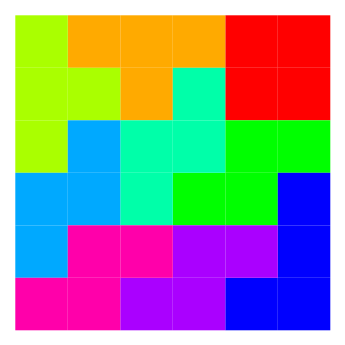
\includegraphics[width=4cm]{tetris.png}
        \end{center}
	
\end{figure}

\section*{Introduction}

Le célèbre jeu Tétris utilise des polygones particuliers formés de petits cubes. Ces polygones sont appelés \emph{polyominos} et peuvent être étudiés d'un point de vue mathématique. C'est le but de ce projet.

\textbf{Mots clés : pavages, combinatoire, géométrie.}

Le principe du projet est d'étudier une question mathématique complexe de façon autonome et originale en utilisant l'outil informatique. \textbf{L'ensemble du projet est à faire par groupe de 3 étudiants.} Le projet est divisé en 2 sections : théorique et pratique. La première partie est \textbf{obligatoire}, la seconde partie correspond à des \textbf{pistes de travail}.

\subsection*{Rendu du projet}\strut

Vous devrez rendre:

\begin{itemize}

\item un \textbf{rapport de mi-projet} répondant aux questions de la section 1;

\item un \textbf{exposé} en fin de projet présentant votre travail et vos résultats sur la section 2.
\end{itemize}

\subsection*{Le rapport}\strut

\smallskip
\textbf{Date de rendu} : cf site du cours \url{https://www.lri.fr/~pons/teaching-mathinfo-l1.html}

\smallskip
\textbf{Que faut-il faire ?} Répondre aux questions de la section 1.

\smallskip
\textbf{Quel format ?} Format PDF obligatoire. Si vous souhaitez ajouter des dessins, vous pouvez les scanner et les ajouter à votre document.

\smallskip
\textbf{Qui réalise le rapport ?} Les membres du groupe réfléchissent ensemble au rapport mais rédigent chacun leur propre rapport. N'oubliez pas de préciser sur votre document qui sont les autres membres du groupe !

\smallskip
\textbf{Comment le rendre ?} Dans votre projet CoCalc, vous trouverez un dossier \og Rapport\fg, c'est là qu'il faut uploader votre rapport PDF.

\subsection*{L'exposé}\strut

\smallskip
\textbf{Quand ?} Les exposés auront lieu courant mai, la date sera précisée ultérieurement.

\smallskip
\textbf{Que doit-on présenter ?} Vous devez présenter le travail effecuté sur la section 2 du projet, en particulier les résultats que vous avez obtenus, les algorithmes que vous avez utilisés, les images ou vidéos produites, etc.

\smallskip
\textbf{En combien de temps ?} Vous aurez 10 minutes de présentation, puis 5 minutes de questions.

\smallskip
\textbf{Sur quel support ?} Vous aurez un vidéo projecteur et un ordinateur à disposition (ou le votre si vous le souhaitez). Vous pourrez donc présenter votre exposé sous forme d'un powerpoint ou pdf. Vous pouvez aussi montrer des images, vidéos, démos de code.

\smallskip
\textbf{Qui parle ?} Tout le monde ! Les 3 étudiants doivent participer.

\smallskip
\textbf{Doit-on présenter notre code ?} Vous pouvez utiliser un notebook CoCalc pour présenter des démos de code, cependant nous ne notons pas la programmation mais bien les résultats obtenus !

\smallskip
\textbf{Doit-on répondre aux questions ?} Les question de la section 2 ne sont pas obligatoires, ce sont des pistes de travail, vous pouvez les suivre, ou pas...


\section{\'Etude théorique du problème}

\subsection{Définition}

Un \emph{polyomino} est une figure plane composée de carrés unitaires ayant au moins un côté commun. La \emph{taille} d'un polyomino est donnée par son nombre de carrés, voir les exemples Figure \ref{fig:ex-polyo}.

\begin{figure}[ht]
\begin{tabular}{ccc}
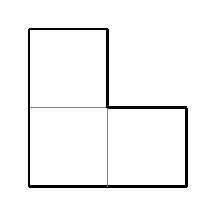
\begin{tikzpicture}
\draw[line width=0.5, color=gray](0,1) -- (1,1);
\draw[line width=1](1,1) -- (1,2);
\draw[line width=1](1,2) -- (0,2);
\draw[line width=1](0,2) -- (0,1);
\draw[line width=1](1,0) -- (2,0);
\draw[line width=1](2,0) -- (2,1);
\draw[line width=1](2,1) -- (1,1);
\draw[line width=1](0,0) -- (1,0);
\draw[line width=0.5, color=gray](1,0) -- (1,1);
\draw[line width=1](0,1) -- (0,0);
\end{tikzpicture}
&
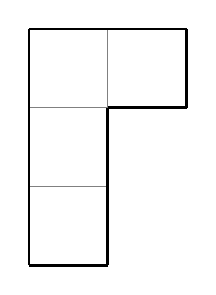
\begin{tikzpicture}
\draw[line width=0.5, color=gray](1,2) -- (2,2);
\draw[line width=0.5, color=gray](2,2) -- (2,3);
\draw[line width=1](2,3) -- (1,3);
\draw[line width=1](1,3) -- (1,2);
\draw[line width=1](1,0) -- (2,0);
\draw[line width=1](2,0) -- (2,1);
\draw[line width=1](1,1) -- (1,0);
\draw[line width=0.5, color=gray](1,1) -- (2,1);
\draw[line width=1](2,1) -- (2,2);
\draw[line width=1](1,2) -- (1,1);
\draw[line width=1](2,2) -- (3,2);
\draw[line width=1](3,2) -- (3,3);
\draw[line width=1](3,3) -- (2,3);
\end{tikzpicture}
&
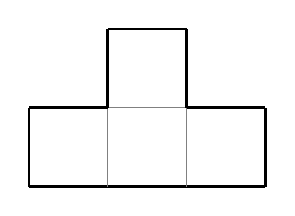
\begin{tikzpicture}
\draw[line width=1](2,0) -- (3,0);
\draw[line width=1](3,0) -- (3,1);
\draw[line width=1](3,1) -- (2,1);
\draw[line width=1](1,0) -- (2,0);
\draw[line width=0.5, color=gray](2,0) -- (2,1);
\draw[line width=1](0,0) -- (1,0);
\draw[line width=0.5, color=gray](1,0) -- (1,1);
\draw[line width=1](1,1) -- (0,1);
\draw[line width=1](0,1) -- (0,0);
\draw[line width=0.5, color=gray](1,1) -- (2,1);
\draw[line width=1](2,1) -- (2,2);
\draw[line width=1](2,2) -- (1,2);
\draw[line width=1](1,2) -- (1,1);
\end{tikzpicture}
\end{tabular}
\caption{Trois polyominos de tailles respectives 3, 4 et 4}
\label{fig:ex-polyo}
\end{figure}

Il y a plusieurs conventions pour décider si deux polyominos sont égaux. Nous travaillons avec la convention la plus simple celle des \emph{polyominos à forme fixée}. Dans ce cas, deux polyominos sont considérés égaux s'ils ont la même forme et tels que les rotations et retournements ne sont pas permis. La Figure~\ref{fig:poly-diff} donne un exemple.

\begin{figure}[ht]
\begin{tabular}{ccc}
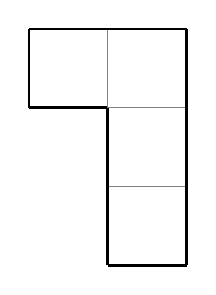
\begin{tikzpicture}
\draw[line width=0.5, color=gray](1,2) -- (2,2);
\draw[line width=1](2,2) -- (2,3);
\draw[line width=1](2,3) -- (1,3);
\draw[line width=1](1,0) -- (2,0);
\draw[line width=1](2,0) -- (2,1);
\draw[line width=1](1,1) -- (1,0);
\draw[line width=0.5, color=gray](1,1) -- (2,1);
\draw[line width=1](2,1) -- (2,2);
\draw[line width=1](1,2) -- (1,1);
\draw[line width=1](0,2) -- (1,2);
\draw[line width=0.5, color=gray](1,2) -- (1,3);
\draw[line width=1](1,3) -- (0,3);
\draw[line width=1](0,3) -- (0,2);
\end{tikzpicture}
&
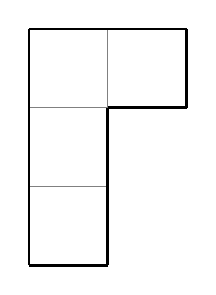
\begin{tikzpicture}
\draw[line width=0.5, color=gray](1,2) -- (2,2);
\draw[line width=0.5, color=gray](2,2) -- (2,3);
\draw[line width=1](2,3) -- (1,3);
\draw[line width=1](1,3) -- (1,2);
\draw[line width=1](1,0) -- (2,0);
\draw[line width=1](2,0) -- (2,1);
\draw[line width=1](1,1) -- (1,0);
\draw[line width=0.5, color=gray](1,1) -- (2,1);
\draw[line width=1](2,1) -- (2,2);
\draw[line width=1](1,2) -- (1,1);
\draw[line width=1](2,2) -- (3,2);
\draw[line width=1](3,2) -- (3,3);
\draw[line width=1](3,3) -- (2,3);
\end{tikzpicture}
&
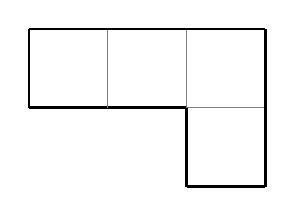
\begin{tikzpicture}
\draw[line width=0.5, color=gray](3,0) -- (4,0);
\draw[line width=1](4,0) -- (4,1);
\draw[line width=1](4,1) -- (3,1);
\draw[line width=1](2,0) -- (3,0);
\draw[line width=0.5, color=gray](3,0) -- (3,1);
\draw[line width=1](3,1) -- (2,1);
\draw[line width=1](1,0) -- (2,0);
\draw[line width=0.5, color=gray](2,0) -- (2,1);
\draw[line width=1](2,1) -- (1,1);
\draw[line width=1](1,1) -- (1,0);
\draw[line width=1](3,-1) -- (4,-1);
\draw[line width=1](4,-1) -- (4,0);
\draw[line width=1](3,0) -- (3,-1);
\end{tikzpicture}
\end{tabular}
\caption{Pour la convention \emph{à forme fixée}, les trois polyominos ci-dessus sont considérés comme différents.}
\label{fig:poly-diff}
\end{figure}

La \emph{classe de rotation} d'un polyomino $P$ est l'ensemble des polyominos que l'on obtient par rotations successives de 45 degrés de $P$. Sa \emph{classe de symétrie} est l'ensemble des polyominos que l'on obtient par symétries successives de  $P$. Enfin, on appellera l'ensemble des polyominos obtenus par rotations ou symétries successive de $P$ la \emph{classe complète} de $P$. Des exemples sont donnés en Figures \ref{fig:rotation}, \ref{fig:symetrie} et \ref{fig:class_complete}.

\begin{figure}[ht]
\begin{tabular}{cccc}
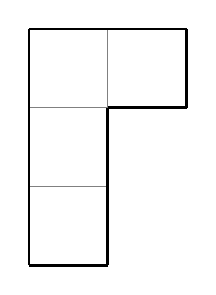
\begin{tikzpicture}
\draw[line width=0.5, color=gray](1,2) -- (2,2);
\draw[line width=0.5, color=gray](2,2) -- (2,3);
\draw[line width=1](2,3) -- (1,3);
\draw[line width=1](1,3) -- (1,2);
\draw[line width=1](1,0) -- (2,0);
\draw[line width=1](2,0) -- (2,1);
\draw[line width=1](1,1) -- (1,0);
\draw[line width=0.5, color=gray](1,1) -- (2,1);
\draw[line width=1](2,1) -- (2,2);
\draw[line width=1](1,2) -- (1,1);
\draw[line width=1](2,2) -- (3,2);
\draw[line width=1](3,2) -- (3,3);
\draw[line width=1](3,3) -- (2,3);
\end{tikzpicture}
&
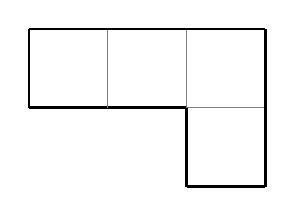
\begin{tikzpicture}
\draw[line width=0.5, color=gray](3,0) -- (4,0);
\draw[line width=1](4,0) -- (4,1);
\draw[line width=1](4,1) -- (3,1);
\draw[line width=1](2,0) -- (3,0);
\draw[line width=0.5, color=gray](3,0) -- (3,1);
\draw[line width=1](3,1) -- (2,1);
\draw[line width=1](1,0) -- (2,0);
\draw[line width=0.5, color=gray](2,0) -- (2,1);
\draw[line width=1](2,1) -- (1,1);
\draw[line width=1](1,1) -- (1,0);
\draw[line width=1](3,-1) -- (4,-1);
\draw[line width=1](4,-1) -- (4,0);
\draw[line width=1](3,0) -- (3,-1);
\end{tikzpicture}
&
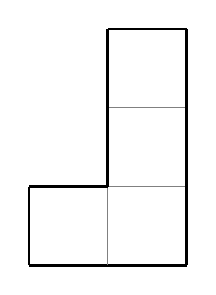
\begin{tikzpicture}
\draw[line width=0.5, color=gray](4,1) -- (5,1);
\draw[line width=1](5,1) -- (5,2);
\draw[line width=1](5,2) -- (4,2);
\draw[line width=1](4,2) -- (4,1);
\draw[line width=1](4,-1) -- (5,-1);
\draw[line width=1](5,-1) -- (5,0);
\draw[line width=1](3,-1) -- (4,-1);
\draw[line width=0.5, color=gray](4,-1) -- (4,0);
\draw[line width=1](4,0) -- (3,0);
\draw[line width=1](3,0) -- (3,-1);
\draw[line width=0.5, color=gray](4,0) -- (5,0);
\draw[line width=1](5,0) -- (5,1);
\draw[line width=1](4,1) -- (4,0);
\end{tikzpicture}
&
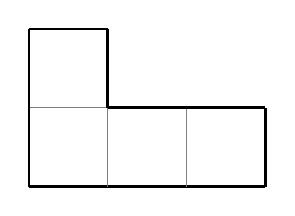
\begin{tikzpicture}
\draw[line width=1](5,-2) -- (6,-2);
\draw[line width=1](6,-2) -- (6,-1);
\draw[line width=1](6,-1) -- (5,-1);
\draw[line width=0.5, color=gray](3,-1) -- (4,-1);
\draw[line width=1](4,-1) -- (4,0);
\draw[line width=1](4,0) -- (3,0);
\draw[line width=1](3,0) -- (3,-1);
\draw[line width=1](3,-2) -- (4,-2);
\draw[line width=0.5, color=gray](4,-2) -- (4,-1);
\draw[line width=1](3,-1) -- (3,-2);
\draw[line width=1](4,-2) -- (5,-2);
\draw[line width=0.5, color=gray](5,-2) -- (5,-1);
\draw[line width=1](5,-1) -- (4,-1);
\end{tikzpicture}
\end{tabular}
\caption{Classe de rotation d'un polyomino}
\label{fig:rotation}
\end{figure}

\begin{figure}[ht]
\begin{tabular}{cc}
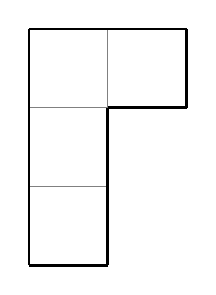
\begin{tikzpicture}
\draw[line width=0.5, color=gray](1,2) -- (2,2);
\draw[line width=0.5, color=gray](2,2) -- (2,3);
\draw[line width=1](2,3) -- (1,3);
\draw[line width=1](1,3) -- (1,2);
\draw[line width=1](1,0) -- (2,0);
\draw[line width=1](2,0) -- (2,1);
\draw[line width=1](1,1) -- (1,0);
\draw[line width=0.5, color=gray](1,1) -- (2,1);
\draw[line width=1](2,1) -- (2,2);
\draw[line width=1](1,2) -- (1,1);
\draw[line width=1](2,2) -- (3,2);
\draw[line width=1](3,2) -- (3,3);
\draw[line width=1](3,3) -- (2,3);
\end{tikzpicture}
&
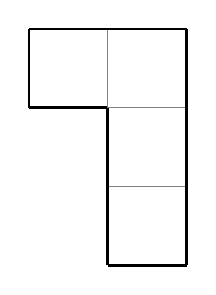
\begin{tikzpicture}
\draw[line width=0.5, color=gray](1,2) -- (2,2);
\draw[line width=1](2,2) -- (2,3);
\draw[line width=1](2,3) -- (1,3);
\draw[line width=1](1,0) -- (2,0);
\draw[line width=1](2,0) -- (2,1);
\draw[line width=1](1,1) -- (1,0);
\draw[line width=0.5, color=gray](1,1) -- (2,1);
\draw[line width=1](2,1) -- (2,2);
\draw[line width=1](1,2) -- (1,1);
\draw[line width=1](0,2) -- (1,2);
\draw[line width=0.5, color=gray](1,2) -- (1,3);
\draw[line width=1](1,3) -- (0,3);
\draw[line width=1](0,3) -- (0,2);
\end{tikzpicture}
\\
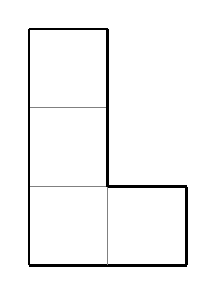
\begin{tikzpicture}
\draw[line width=1](0,-2) -- (1,-2);
\draw[line width=1](1,-2) -- (1,-1);
\draw[line width=1](1,-1) -- (0,-1);
\draw[line width=0.5, color=gray](-1,-1) -- (0,-1);
\draw[line width=1](0,-1) -- (0,0);
\draw[line width=1](-1,0) -- (-1,-1);
\draw[line width=0.5, color=gray](-1,0) -- (0,0);
\draw[line width=1](0,0) -- (0,1);
\draw[line width=1](0,1) -- (-1,1);
\draw[line width=1](-1,1) -- (-1,0);
\draw[line width=1](-1,-2) -- (0,-2);
\draw[line width=0.5, color=gray](0,-2) -- (0,-1);
\draw[line width=1](-1,-1) -- (-1,-2);
\end{tikzpicture}
&

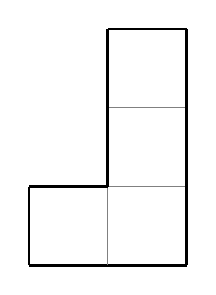
\begin{tikzpicture}
\draw[line width=0.5, color=gray](1,-1) -- (2,-1);
\draw[line width=1](2,-1) -- (2,0);
\draw[line width=1](1,0) -- (1,-1);
\draw[line width=0.5, color=gray](1,0) -- (2,0);
\draw[line width=1](2,0) -- (2,1);
\draw[line width=1](2,1) -- (1,1);
\draw[line width=1](1,1) -- (1,0);
\draw[line width=1](1,-2) -- (2,-2);
\draw[line width=1](2,-2) -- (2,-1);
\draw[line width=1](0,-2) -- (1,-2);
\draw[line width=0.5, color=gray](1,-2) -- (1,-1);
\draw[line width=1](1,-1) -- (0,-1);
\draw[line width=1](0,-1) -- (0,-2);
\end{tikzpicture}
\end{tabular}
\caption{Classe de symétrie d'un polyomino}
\label{fig:symetrie}
\end{figure}

\begin{figure}[ht]
\begin{tabular}{cccc}
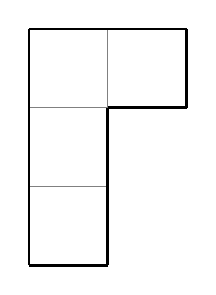
\begin{tikzpicture}
\draw[line width=0.5, color=gray](1,2) -- (2,2);
\draw[line width=0.5, color=gray](2,2) -- (2,3);
\draw[line width=1](2,3) -- (1,3);
\draw[line width=1](1,3) -- (1,2);
\draw[line width=1](1,0) -- (2,0);
\draw[line width=1](2,0) -- (2,1);
\draw[line width=1](1,1) -- (1,0);
\draw[line width=0.5, color=gray](1,1) -- (2,1);
\draw[line width=1](2,1) -- (2,2);
\draw[line width=1](1,2) -- (1,1);
\draw[line width=1](2,2) -- (3,2);
\draw[line width=1](3,2) -- (3,3);
\draw[line width=1](3,3) -- (2,3);
\end{tikzpicture}
&
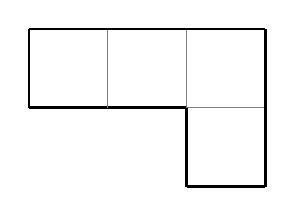
\begin{tikzpicture}
\draw[line width=0.5, color=gray](3,0) -- (4,0);
\draw[line width=1](4,0) -- (4,1);
\draw[line width=1](4,1) -- (3,1);
\draw[line width=1](2,0) -- (3,0);
\draw[line width=0.5, color=gray](3,0) -- (3,1);
\draw[line width=1](3,1) -- (2,1);
\draw[line width=1](1,0) -- (2,0);
\draw[line width=0.5, color=gray](2,0) -- (2,1);
\draw[line width=1](2,1) -- (1,1);
\draw[line width=1](1,1) -- (1,0);
\draw[line width=1](3,-1) -- (4,-1);
\draw[line width=1](4,-1) -- (4,0);
\draw[line width=1](3,0) -- (3,-1);
\end{tikzpicture}
&
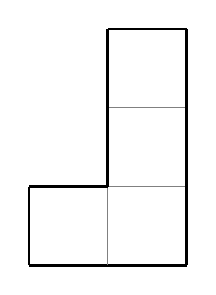
\begin{tikzpicture}
\draw[line width=0.5, color=gray](4,1) -- (5,1);
\draw[line width=1](5,1) -- (5,2);
\draw[line width=1](5,2) -- (4,2);
\draw[line width=1](4,2) -- (4,1);
\draw[line width=1](4,-1) -- (5,-1);
\draw[line width=1](5,-1) -- (5,0);
\draw[line width=1](3,-1) -- (4,-1);
\draw[line width=0.5, color=gray](4,-1) -- (4,0);
\draw[line width=1](4,0) -- (3,0);
\draw[line width=1](3,0) -- (3,-1);
\draw[line width=0.5, color=gray](4,0) -- (5,0);
\draw[line width=1](5,0) -- (5,1);
\draw[line width=1](4,1) -- (4,0);
\end{tikzpicture}
&
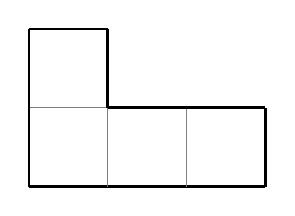
\begin{tikzpicture}
\draw[line width=1](5,-2) -- (6,-2);
\draw[line width=1](6,-2) -- (6,-1);
\draw[line width=1](6,-1) -- (5,-1);
\draw[line width=0.5, color=gray](3,-1) -- (4,-1);
\draw[line width=1](4,-1) -- (4,0);
\draw[line width=1](4,0) -- (3,0);
\draw[line width=1](3,0) -- (3,-1);
\draw[line width=1](3,-2) -- (4,-2);
\draw[line width=0.5, color=gray](4,-2) -- (4,-1);
\draw[line width=1](3,-1) -- (3,-2);
\draw[line width=1](4,-2) -- (5,-2);
\draw[line width=0.5, color=gray](5,-2) -- (5,-1);
\draw[line width=1](5,-1) -- (4,-1);
\end{tikzpicture}
\\
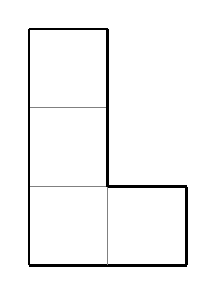
\begin{tikzpicture}
\draw[line width=0.5, color=gray](1,-1) -- (2,-1);
\draw[line width=1](2,-1) -- (2,0);
\draw[line width=1](1,0) -- (1,-1);
\draw[line width=0.5, color=gray](1,0) -- (2,0);
\draw[line width=1](2,0) -- (2,1);
\draw[line width=1](2,1) -- (1,1);
\draw[line width=1](1,1) -- (1,0);
\draw[line width=1](2,-2) -- (3,-2);
\draw[line width=1](3,-2) -- (3,-1);
\draw[line width=1](3,-1) -- (2,-1);
\draw[line width=1](1,-2) -- (2,-2);
\draw[line width=0.5, color=gray](2,-2) -- (2,-1);
\draw[line width=1](1,-1) -- (1,-2);
\end{tikzpicture}
&
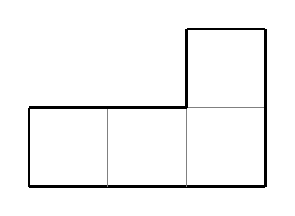
\begin{tikzpicture}
\draw[line width=1](2,-2) -- (3,-2);
\draw[line width=0.5, color=gray](3,-2) -- (3,-1);
\draw[line width=1](3,-1) -- (2,-1);
\draw[line width=1](1,-2) -- (2,-2);
\draw[line width=0.5, color=gray](2,-2) -- (2,-1);
\draw[line width=1](2,-1) -- (1,-1);
\draw[line width=1](1,-1) -- (1,-2);
\draw[line width=0.5, color=gray](3,-1) -- (4,-1);
\draw[line width=1](4,-1) -- (4,0);
\draw[line width=1](4,0) -- (3,0);
\draw[line width=1](3,0) -- (3,-1);
\draw[line width=1](3,-2) -- (4,-2);
\draw[line width=1](4,-2) -- (4,-1);
\end{tikzpicture}
&
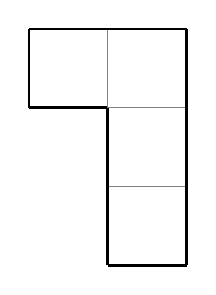
\begin{tikzpicture}
\draw[line width=1](4,-3) -- (5,-3);
\draw[line width=1](5,-3) -- (5,-2);
\draw[line width=1](4,-2) -- (4,-3);
\draw[line width=0.5, color=gray](4,-1) -- (5,-1);
\draw[line width=1](5,-1) -- (5,0);
\draw[line width=1](5,0) -- (4,0);
\draw[line width=1](3,-1) -- (4,-1);
\draw[line width=0.5, color=gray](4,-1) -- (4,0);
\draw[line width=1](4,0) -- (3,0);
\draw[line width=1](3,0) -- (3,-1);
\draw[line width=0.5, color=gray](4,-2) -- (5,-2);
\draw[line width=1](5,-2) -- (5,-1);
\draw[line width=1](4,-1) -- (4,-2);
\end{tikzpicture}
&
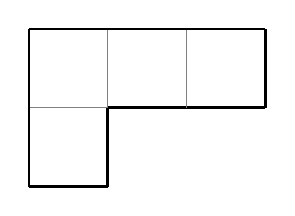
\begin{tikzpicture}
\draw[line width=1](5,-2) -- (6,-2);
\draw[line width=1](6,-2) -- (6,-1);
\draw[line width=1](6,-1) -- (5,-1);
\draw[line width=1](4,-2) -- (5,-2);
\draw[line width=0.5, color=gray](5,-2) -- (5,-1);
\draw[line width=1](5,-1) -- (4,-1);
\draw[line width=0.5, color=gray](3,-2) -- (4,-2);
\draw[line width=0.5, color=gray](4,-2) -- (4,-1);
\draw[line width=1](4,-1) -- (3,-1);
\draw[line width=1](3,-1) -- (3,-2);
\draw[line width=1](3,-3) -- (4,-3);
\draw[line width=1](4,-3) -- (4,-2);
\draw[line width=1](3,-2) -- (3,-3);
\end{tikzpicture}
\end{tabular}
\caption{Classe complète d'un polyomino}
\label{fig:class_complete}
\end{figure}

\subsection{Questions}

\begin{enumerate}
\item Donnez les classes de rotation, de symétrie et classes complètes des deux polyominos suivants.

\begin{tabular}{cc}
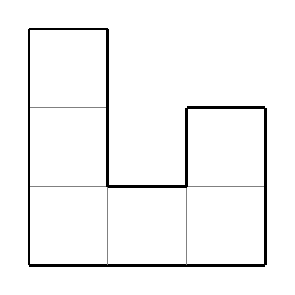
\begin{tikzpicture}
\draw[line width=0.5, color=gray](0,1) -- (1,1);
\draw[line width=1](1,1) -- (1,2);
\draw[line width=1](0,2) -- (0,1);
\draw[line width=1](0,0) -- (1,0);
\draw[line width=0.5, color=gray](1,0) -- (1,1);
\draw[line width=1](0,1) -- (0,0);
\draw[line width=0.5, color=gray](2,1) -- (3,1);
\draw[line width=1](3,1) -- (3,2);
\draw[line width=1](3,2) -- (2,2);
\draw[line width=1](2,2) -- (2,1);
\draw[line width=1](2,0) -- (3,0);
\draw[line width=1](3,0) -- (3,1);
\draw[line width=1](1,0) -- (2,0);
\draw[line width=0.5, color=gray](2,0) -- (2,1);
\draw[line width=1](2,1) -- (1,1);
\draw[line width=0.5, color=gray](0,2) -- (1,2);
\draw[line width=1](1,2) -- (1,3);
\draw[line width=1](1,3) -- (0,3);
\draw[line width=1](0,3) -- (0,2);
\end{tikzpicture}
&
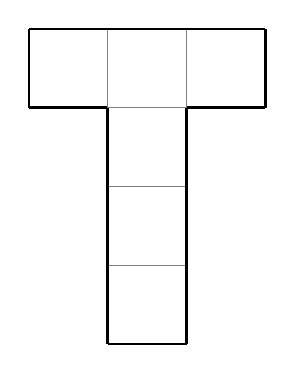
\begin{tikzpicture}
\draw[line width=0.5, color=gray](0,1) -- (1,1);
\draw[line width=1](1,1) -- (1,2);
\draw[line width=1](0,2) -- (0,1);
\draw[line width=1](0,0) -- (1,0);
\draw[line width=1](1,0) -- (1,1);
\draw[line width=1](0,1) -- (0,0);
\draw[line width=1](-1,3) -- (0,3);
\draw[line width=0.5, color=gray](0,3) -- (0,4);
\draw[line width=1](0,4) -- (-1,4);
\draw[line width=1](-1,4) -- (-1,3);
\draw[line width=1](1,3) -- (2,3);
\draw[line width=1](2,3) -- (2,4);
\draw[line width=1](2,4) -- (1,4);
\draw[line width=0.5, color=gray](0,3) -- (1,3);
\draw[line width=0.5, color=gray](1,3) -- (1,4);
\draw[line width=1](1,4) -- (0,4);
\draw[line width=0.5, color=gray](0,2) -- (1,2);
\draw[line width=1](1,2) -- (1,3);
\draw[line width=1](0,3) -- (0,2);
\end{tikzpicture}
\end{tabular}

\item Combien d'éléments une classe de rotation peut-elle contenir au maximum ? Justifiez la réponse et donnez un exemple où le maximum n'est pas atteint.

\item Même question pour une classe complète.

\item Donnez tous les polyominos de tailles 4 en distinguant les différentes classes complètes et classes de rotation. Vous devez trouver 19 polyominos, 7 classes de rotations et 5 classes complètes.

\item Donnez les 12 classes complètes de polyominos de taille 5 (pour chaque classe, vous pouvez ne dessiner qu'un seul polyomino). 

\item La question la plus classique sur les polyominos est celle du \emph{pavage} : recouvrir complètement une zone du plan (ou le plan entier) par des polyominos. Un exemple de pavage est donné en Figure \ref{fig:ex-pavage}. Donnez un autre pavage du carré $6 \times 6$ par des polyominos de taille 4.

\item Prouvez qu'il n'est pas possible de paver un rectangle avec le polyomino suivant. Cependant, expliquez comment vous pourriez paver un plan infini.

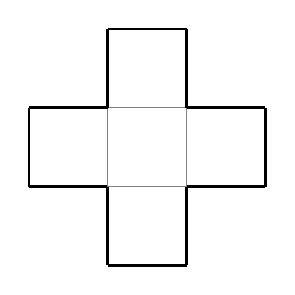
\begin{tikzpicture}
\draw[line width=0.5, color=gray](0,1) -- (1,1);
\draw[line width=0.5, color=gray](1,1) -- (1,2);
\draw[line width=1](-1,1) -- (0,1);
\draw[line width=0.5, color=gray](0,1) -- (0,2);
\draw[line width=1](0,2) -- (-1,2);
\draw[line width=1](-1,2) -- (-1,1);
\draw[line width=1](0,0) -- (1,0);
\draw[line width=1](1,0) -- (1,1);
\draw[line width=1](0,1) -- (0,0);
\draw[line width=0.5, color=gray](0,2) -- (1,2);
\draw[line width=1](1,2) -- (1,3);
\draw[line width=1](1,3) -- (0,3);
\draw[line width=1](0,3) -- (0,2);
\draw[line width=1](1,1) -- (2,1);
\draw[line width=1](2,1) -- (2,2);
\draw[line width=1](2,2) -- (1,2);
\end{tikzpicture}

\item Prouvez qu'il est possible de paver n'importe quel rectangle $2n \times 4m$ avec les polyominos de la classe représentée en Figure \ref{fig:class_complete}. 

\item On peut aussi s'intéresser au nombre de pavages possibles. Soit une ligne de hauteur 1 et de longueur $n$. On possède deux polyominos : un de taille 1 composé d'un unique carré et un de taille 2 composé de deux carrés consécutifs. Donnez les pavages possibles pour $n = 1, 2, 3, 4, 5$ ? Reconnaissez-vous ces nombres ?
\end{enumerate}

\begin{figure}[ht]
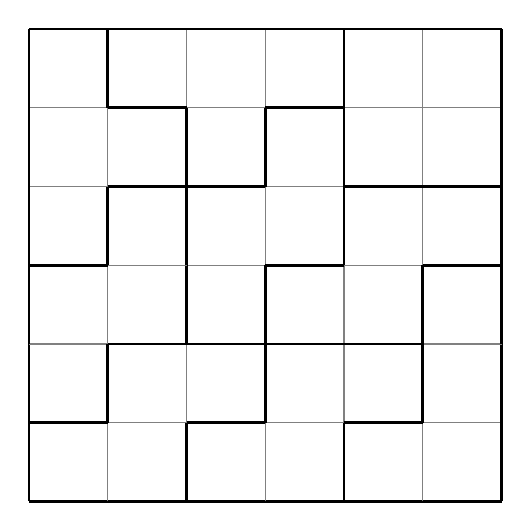
\begin{tikzpicture}
\draw[line width=0.5, color=gray](4,5) -- (5,5);
\draw[line width=0.5, color=gray](5,5) -- (5,6);
\draw[line width=1](5,6) -- (4,6);
\draw[line width=1](4,6) -- (4,5);
\draw[line width=1](5,4) -- (6,4);
\draw[line width=1](6,4) -- (6,5);
\draw[line width=1](4,4) -- (5,4);
\draw[line width=0.5, color=gray](5,4) -- (5,5);
\draw[line width=1](4,5) -- (4,4);
\draw[line width=0.5, color=gray](5,5) -- (6,5);
\draw[line width=1](6,5) -- (6,6);
\draw[line width=1](6,6) -- (5,6);

\draw[line width=1](1,5) -- (2,5);
\draw[line width=0.5, color=gray](2,5) -- (2,6);
\draw[line width=1](2,6) -- (1,6);
\draw[line width=1](1,6) -- (1,5);
\draw[line width=0.5, color=gray](2,5) -- (3,5);
\draw[line width=0.5, color=gray](3,5) -- (3,6);
\draw[line width=1](3,6) -- (2,6);
\draw[line width=1](2,4) -- (3,4);
\draw[line width=1](3,4) -- (3,5);
\draw[line width=1](2,5) -- (2,4);
\draw[line width=1](3,5) -- (4,5);
\draw[line width=1](4,5) -- (4,6);
\draw[line width=1](4,6) -- (3,6);

\draw[line width=1](0,3) -- (1,3);
\draw[line width=1](1,3) -- (1,4);
\draw[line width=1](0,4) -- (0,3);
\draw[line width=0.5, color=gray](0,5) -- (1,5);
\draw[line width=1](1,5) -- (1,6);
\draw[line width=1](1,6) -- (0,6);
\draw[line width=1](0,6) -- (0,5);
\draw[line width=1](1,4) -- (2,4);
\draw[line width=1](2,4) -- (2,5);
\draw[line width=1](2,5) -- (1,5);
\draw[line width=0.5, color=gray](0,4) -- (1,4);
\draw[line width=0.5, color=gray](1,4) -- (1,5);
\draw[line width=1](0,5) -- (0,4);

\draw[line width=1](4,2) -- (5,2);
\draw[line width=1](5,2) -- (5,3);
\draw[line width=1](3,2) -- (4,2);
\draw[line width=0.5, color=gray](4,2) -- (4,3);
\draw[line width=1](4,3) -- (3,3);
\draw[line width=1](3,3) -- (3,2);
\draw[line width=0.5, color=gray](4,3) -- (5,3);
\draw[line width=0.5, color=gray](5,3) -- (5,4);
\draw[line width=1](5,4) -- (4,4);
\draw[line width=1](4,4) -- (4,3);
\draw[line width=1](5,3) -- (6,3);
\draw[line width=1](6,3) -- (6,4);
\draw[line width=1](6,4) -- (5,4);

\draw[line width=0.5, color=gray](3,4) -- (4,4);
\draw[line width=1](4,4) -- (4,5);
\draw[line width=1](4,5) -- (3,5);
\draw[line width=1](3,5) -- (3,4);
\draw[line width=0.5, color=gray](2,3) -- (3,3);
\draw[line width=0.5, color=gray](3,3) -- (3,4);
\draw[line width=1](3,4) -- (2,4);
\draw[line width=1](2,4) -- (2,3);
\draw[line width=1](3,3) -- (4,3);
\draw[line width=1](4,3) -- (4,4);
\draw[line width=1](2,2) -- (3,2);
\draw[line width=1](3,2) -- (3,3);
\draw[line width=1](2,3) -- (2,2);

\draw[line width=1](0,1) -- (1,1);
\draw[line width=1](1,1) -- (1,2);
\draw[line width=1](0,2) -- (0,1);
\draw[line width=1](1,2) -- (2,2);
\draw[line width=1](2,2) -- (2,3);
\draw[line width=0.5, color=gray](1,3) -- (2,3);
\draw[line width=1](2,3) -- (2,4);
\draw[line width=1](2,4) -- (1,4);
\draw[line width=1](1,4) -- (1,3);
\draw[line width=0.5, color=gray](0,2) -- (1,2);
\draw[line width=0.5, color=gray](1,2) -- (1,3);
\draw[line width=1](1,3) -- (0,3);
\draw[line width=1](0,3) -- (0,2);

\draw[line width=0.5, color=gray](5,1) -- (6,1);
\draw[line width=1](6,1) -- (6,2);
\draw[line width=1](5,2) -- (5,1);
\draw[line width=0.5, color=gray](5,2) -- (6,2);
\draw[line width=1](6,2) -- (6,3);
\draw[line width=1](6,3) -- (5,3);
\draw[line width=1](5,3) -- (5,2);
\draw[line width=1](5,0) -- (6,0);
\draw[line width=1](6,0) -- (6,1);
\draw[line width=1](4,0) -- (5,0);
\draw[line width=0.5, color=gray](5,0) -- (5,1);
\draw[line width=1](5,1) -- (4,1);
\draw[line width=1](4,1) -- (4,0);

\draw[line width=1](3,0) -- (4,0);
\draw[line width=1](4,0) -- (4,1);
\draw[line width=1](2,0) -- (3,0);
\draw[line width=0.5, color=gray](3,0) -- (3,1);
\draw[line width=1](3,1) -- (2,1);
\draw[line width=1](2,1) -- (2,0);
\draw[line width=0.5, color=gray](3,1) -- (4,1);
\draw[line width=0.5, color=gray](4,1) -- (4,2);
\draw[line width=1](4,2) -- (3,2);
\draw[line width=1](3,2) -- (3,1);
\draw[line width=1](4,1) -- (5,1);
\draw[line width=1](5,1) -- (5,2);
\draw[line width=1](5,2) -- (4,2);

\draw[line width=1](1,0) -- (2,0);
\draw[line width=1](2,0) -- (2,1);
\draw[line width=1](0,0) -- (1,0);
\draw[line width=0.5, color=gray](1,0) -- (1,1);
\draw[line width=1](1,1) -- (0,1);
\draw[line width=1](0,1) -- (0,0);
\draw[line width=0.5, color=gray](1,1) -- (2,1);
\draw[line width=0.5, color=gray](2,1) -- (2,2);
\draw[line width=1](2,2) -- (1,2);
\draw[line width=1](1,2) -- (1,1);
\draw[line width=1](2,1) -- (3,1);
\draw[line width=1](3,1) -- (3,2);
\draw[line width=1](3,2) -- (2,2);
\end{tikzpicture}

\caption{Pavage d'un carré $6 \times 6$ par des polyominos de taille 4}
\label{fig:ex-pavage}
\end{figure}

\section{Modélisation et exploration}

Le but de cette partie est d'explorer les questions relatives aux polyominos avec l'aide de l'outil informatique. Nous vous proposons ici des pistes, à vous de les explorer ou d'en proposer de nouvelles.

\subsection{Modélisation et visualisation}

Le but de cette section est de représenter et traiter les polyominos en tant qu'objet informatique.

\begin{enumerate}
\item Proposez une ou des solutions pour représenter les polyominos en tant qu'objet informatique.

\item Comment obtenir les classes de rotation et de symétrie d'un polyomino donné ?

\item Comment tester que deux polyominos appartiennent à la même classe complète ?

\item Comment représenter le pavage d'une zone donnée ?

\item Proposez des fonctions d'affichage (avec {\tt plot}) pour représenter les polyominos et les pavages.
\end{enumerate}

\subsection{Pavages}

Le but de cette section est d'explorer automatiquement les pavages de rectangles par un ensemble de polyominos donnés. 

\begin{enumerate}

\item \textbf{1 seule dimension} On se place d'abord dans un espace à paver d'une seule dimension (un rectangle de longueur $n$ et de hauteur 1). Proposez un algorithme permettant de tester si la ligne peut être pavée par un ensemble de polyominos donnés. Si oui, il faudra donner la solution.

\item \textbf{2 dimensions} Proposez un algorithme permettant de tester si un rectangle donné peut être pavé par un ensemble de polyominos donnés. 

\item Testez votre algorithme sur différents rectangles et ensemble de polyominos. Le but est comprendre quels rectangle peuvent être pavés par un ensemble donné. Exemple d'ensembles : tous les polyominos de taille 4, une classe complète pour un polyomino donné etc.

\item Essayez de prouver certains des résultats que vous obtenez de façon expérimentale.

\item Adaptez votre algorithme à des formes différentes (pas des rectangles).

\item Comment faire pour rechercher des pavages du plan entier ?

\end{enumerate}

\subsection{Génération des polyominos}

Comment engendrer l'ensemble des polyominos ? 

\begin{enumerate}
\item Commencez par générer les polyominos à forme fixée. Vous pouvez soit définir votre propre algorithme, soit implantez des algorithmes existants décrits en particulier sur wikipedia.

\item Comment adapter cet algorithme pour la génération des classes rotations ou classes complètes ?
\end{enumerate}


\subsection{Spécial Tétris}

On se place dans la situation suivante : on a un rectangle et un ensemble de polyominos donnés. A chaque étape, on reçoit un polyomino au hasard qui ne peut être placé "qu'en bas" du rectangle. Si une ligne complète est formée, elle disparaît et toutes les autres lignes descendent d'un cran. Le but n'est pas de jouer mais de chercher un algorithme optimal !


\begin{enumerate}
\item On part du principe que le polyomino envoyé est à forme fixe (on effectue pas de rotation), proposez un algorithme pour le placer de façon optimale et effectuez des tests sur divers rectangles et ensemble de polyominos.

\item Même question avec rotation autorisée.

\item Même question avec symétrie et rotation.

\end{enumerate}

\end{document}



